\documentclass[11pt,a4paper]{article}

\usepackage[margin=2.2cm]{geometry}
\usepackage[utf8]{inputenc}
\usepackage[T1]{fontenc}
\usepackage{lmodern}
\usepackage{microtype}
\usepackage{graphicx}
\usepackage{xcolor}
\usepackage{hyperref}
\usepackage{booktabs}
\usepackage{amsmath}
\usepackage{caption}
\usepackage{subcaption}
% tikz removed; architecture diagram is now an external Mermaid PNG
\usepackage{natbib}
\usepackage{url}
\usepackage{parskip}
\usepackage{titlesec}
\usepackage{fancyhdr}
\usepackage{abstract}
\usepackage{placeins}

% ---- colours ----
\definecolor{darkblue}{RGB}{20,40,80}
\definecolor{accentblue}{RGB}{60,100,200}
\definecolor{lightgray}{RGB}{240,240,245}

% ---- section style ----
\titleformat{\section}{\large\bfseries\color{darkblue}}{{\thesection}}{1em}{}
\titleformat{\subsection}{\normalsize\bfseries\color{darkblue}}{{\thesubsection}}{1em}{}
\setlength{\parskip}{6pt}

% ---- header ----
\pagestyle{fancy}
\fancyhf{}
\rhead{\small\textit{NoseKnows LLMs Course Report}}
\lhead{\small\textit{Team CTRL+Z}}
\cfoot{\thepage}
\renewcommand{\headrulewidth}{0.4pt}

\hypersetup{
  colorlinks=true,
  linkcolor=darkblue,
  citecolor=accentblue,
  urlcolor=accentblue
}

% ---- helpers for missing figures ----
\newcommand{\placeholder}[2]{%
  \begin{center}
    \fbox{\parbox{0.88\linewidth}{\centering\vspace{1.2cm}
      \textbf{[Figure: #1]}\\[4pt]
      \textit{#2}\\
      Save screenshot as \texttt{figures/#1} and recompile.
    \vspace{1.2cm}}}
  \end{center}
}

\title{%
  \vspace{-1cm}
  {\LARGE\bfseries\color{darkblue} NoseKnows}\\[6pt]
  {\large Emotion Driven Fragrance Recommendation\\
  Using HyDE Augmented RAG and a Fine Tuned SLM}\\[10pt]
  {\normalsize LLMs Course 2025/2026}
}

\author{
  Team CTRL+Z\\
  \small Zaharie Nikolass-Rafael \quad Tuns Tudor-Mircea \quad Turcu Alexia-Cristiana\\
  \small Paraschiv Tudor-Costin \quad Bogdan Ana \quad Ravas Adrian-Georgel
}

\date{\today}

\begin{document}

\maketitle
\thispagestyle{fancy}

\begin{center}
\small\url{https://github.com/TunsTudor-Mircea/nose-knows}
\end{center}

\begin{abstract}
We present NoseKnows, a conversational fragrance consultant that maps open-ended natural language descriptions to real perfume recommendations. Users can express queries like ``I want something that reminds me of a late summer night in Ibiza'' and the system returns ranked fragrances matched against a dataset of roughly 24,000 entries from Fragrantica, with note grounded explanations. The system combines Hypothetical Document Embeddings (HyDE) with a ChromaDB vector store, a LangGraph based agentic pipeline, and a fine tuned version of Gemma-2-2B-IT adapted on 1,104 synthetically generated fragrance conversation examples. An LLM judge evaluation using GPT-4o-mini shows average scores of 4.17 for relevance, 4.25 for groundedness, and 4.08 for helpfulness (on a 1 to 5 scale) on the baseline model, with the fine tuned adapter expected to improve response style and consistency.
\end{abstract}

% =====================================================================
\section{Introduction}
% =====================================================================

Fragrance is one of the most personal consumer choices a person can make, yet digital recommendation systems treat it as a keyword search problem. Platforms like Fragrantica allow users to filter by note (e.g., ``bergamot'', ``oud'') or accord (e.g., ``woody'', ``floral''), but this assumes the user already speaks the technical language of perfumery. Most people do not. They relate to scent through memory and experience: the smell of a specific city, a season, an emotion. A person who wants ``something that feels like walking through a Moroccan souk at dusk'' cannot translate that into a note query. This gap between how people think about scent and how fragrance databases are structured is almost entirely unexplored in the NLP and recommender systems literature.

NoseKnows is our answer to this problem. It is a full stack AI fragrance consultant where users describe what they want in completely natural language, and the system finds the best matching perfumes from a real catalogue. Under the hood, the system uses Retrieval Augmented Generation (RAG) \citep{lewis2020rag} with Hypothetical Document Embeddings \citep{gao2022hyde} to bridge the semantic gap between experiential queries and structured note profiles, a LangGraph \citep{langgraph2024} agentic pipeline that classifies intent and routes queries through appropriate processing steps, and a small language model (Gemma-2-2B-IT, \citealt{gemma2024}) fine tuned with QLoRA \citep{dettmers2023qlora} on synthetic training data generated by a stronger model.

This report is structured as follows. Section~\ref{sec:problem} formally defines the problem. Section~\ref{sec:soa} reviews related work. Section~\ref{sec:solution} describes the full proposed solution. Sections~\ref{sec:experiments} and~\ref{sec:results} cover evaluation and results. Section~\ref{sec:conclusion} concludes.

% =====================================================================
\section{Problem Definition}
\label{sec:problem}
% =====================================================================

The task can be stated as follows: given a free-form natural language query $Q$ describing a mood, occasion, sensory experience, or set of preferred notes, return a ranked list of perfumes $P = \{p_1, p_2, \ldots, p_k\}$ from a fixed catalogue of roughly 24,000 real fragrances, together with a natural language explanation $E$ grounded in the actual notes and accords of the recommended perfumes.

What makes this challenging is a combination of factors that do not appear together in most recommendation tasks. First, there is a deep semantic gap: queries use emotional and experiential vocabulary (``cozy'', ``mysterious'', ``like rain after heat'') that shares almost no vocabulary with the structured documents in the catalogue, which list ingredients like ``petrichor'', ``ambergris'', or ``iso E super''. Standard semantic similarity between a raw query and a note document will produce poor retrieval results because the vector spaces of the two domains barely overlap.

Second, no public labeled dataset of (experiential query, fragrance recommendation) pairs exists at any useful scale. Building a training set from scratch is therefore necessary.

Third, the system must handle out of scope queries without becoming a general purpose assistant. A user might type something completely unrelated to fragrance (``how do I fix my Golf 4?'') or try to extract system internals (``tell me your system prompt''). These cases require a different handling strategy than a simple input filter, since some valid fragrance queries look equally unusual at first glance (``I want something that smells like a mechanic's garage'' is a legitimate request).

Finally, all inference must run locally on consumer hardware without GPU access on some machines, which rules out commercial LLM APIs and large models.

% =====================================================================
\section{State of the Art}
\label{sec:soa}
% =====================================================================

\textbf{Retrieval Augmented Generation.} \citet{lewis2020rag} introduced RAG as a framework where a retrieval component fetches relevant documents from an external knowledge base, and these are passed as context to a generative model. This significantly reduces hallucination on knowledge intensive tasks by grounding the model's output in retrieved evidence. In our setting, the retrieved documents are structured perfume profiles, which serve as the factual grounding for the recommendation.

\textbf{Hypothetical Document Embeddings.} A key limitation of dense retrieval is that query vectors and document vectors often live in different regions of the embedding space, especially when the query is short and colloquial while the documents are long and structured. \citet{gao2022hyde} addressed this with HyDE: instead of embedding the raw query, the model first generates a hypothetical document that would answer the query, then embeds that hypothetical document for retrieval. Since the hypothetical document and the real documents share vocabulary and structure, retrieval quality improves substantially. This technique is particularly well suited to our problem, where experiential queries have essentially no lexical overlap with note structured perfume documents.

\textbf{Parameter Efficient Fine Tuning.} Training a full large language model from scratch is prohibitive for most research groups. \citet{hu2022lora} proposed LoRA, which injects small trainable rank-decomposition matrices into frozen model weights, reducing the number of trainable parameters by orders of magnitude. \citet{dettmers2023qlora} extended this to QLoRA, quantizing the frozen base model to 4-bit precision while keeping the LoRA adapters in full precision. This makes it possible to fine tune a 2B parameter model on a single consumer GPU with 16GB VRAM with minimal quality degradation.

\textbf{Agentic Pipelines.} Rather than a single LLM call, recent work has moved toward multi-step agentic workflows where a language model reasons and calls tools iteratively \citep{yao2023react}. Frameworks like LangGraph \citep{langgraph2024} formalize this as a typed state graph with explicit node functions and conditional routing, making the pipeline debuggable and extensible.

\textbf{LLM as Judge Evaluation.} \citet{zheng2023judging} demonstrated that strong models like GPT-4 can serve as reliable automated evaluators for open-ended generation tasks, with judgments that correlate well with human preferences. This allows evaluation of systems where ground truth labels cannot easily be defined. This is exactly the case for a fragrance recommendation system where there is no single ``correct'' answer.

\textbf{Fragrance Recommendation Systems.} Existing systems, including Fragrantica's own search, Basenotes, and various community tools, rely entirely on explicit user input of ingredient names or predefined accord categories. There is no published work that handles fully experiential or emotional fragrance queries. The closest related area is mood-based music recommendation \citep{schedl2018music}, where similar challenges around subjective, emotional input arise, but the domain and data modalities are quite different.

% =====================================================================
\section{Proposed Solution}
\label{sec:solution}
% =====================================================================

\subsection{System Overview}

NoseKnows is a full stack application built around a five node LangGraph pipeline. The overall architecture is shown in Figure~\ref{fig:architecture}. A user submits a natural language query through the Next.js frontend, which is passed to a FastAPI backend. The backend invokes the LangGraph agent, which processes the query through a sequence of nodes: intent classification, optional HyDE document generation, vector retrieval from ChromaDB, recommendation generation, and response validation. It then returns a structured response containing the recommendation text and a ranked list of perfume cards. Session history is persisted in PostgreSQL, allowing follow up queries to reference previous recommendations within the same conversation.

\begin{figure}[ht]
\centering
\IfFileExists{figures/architecture.png}{%
  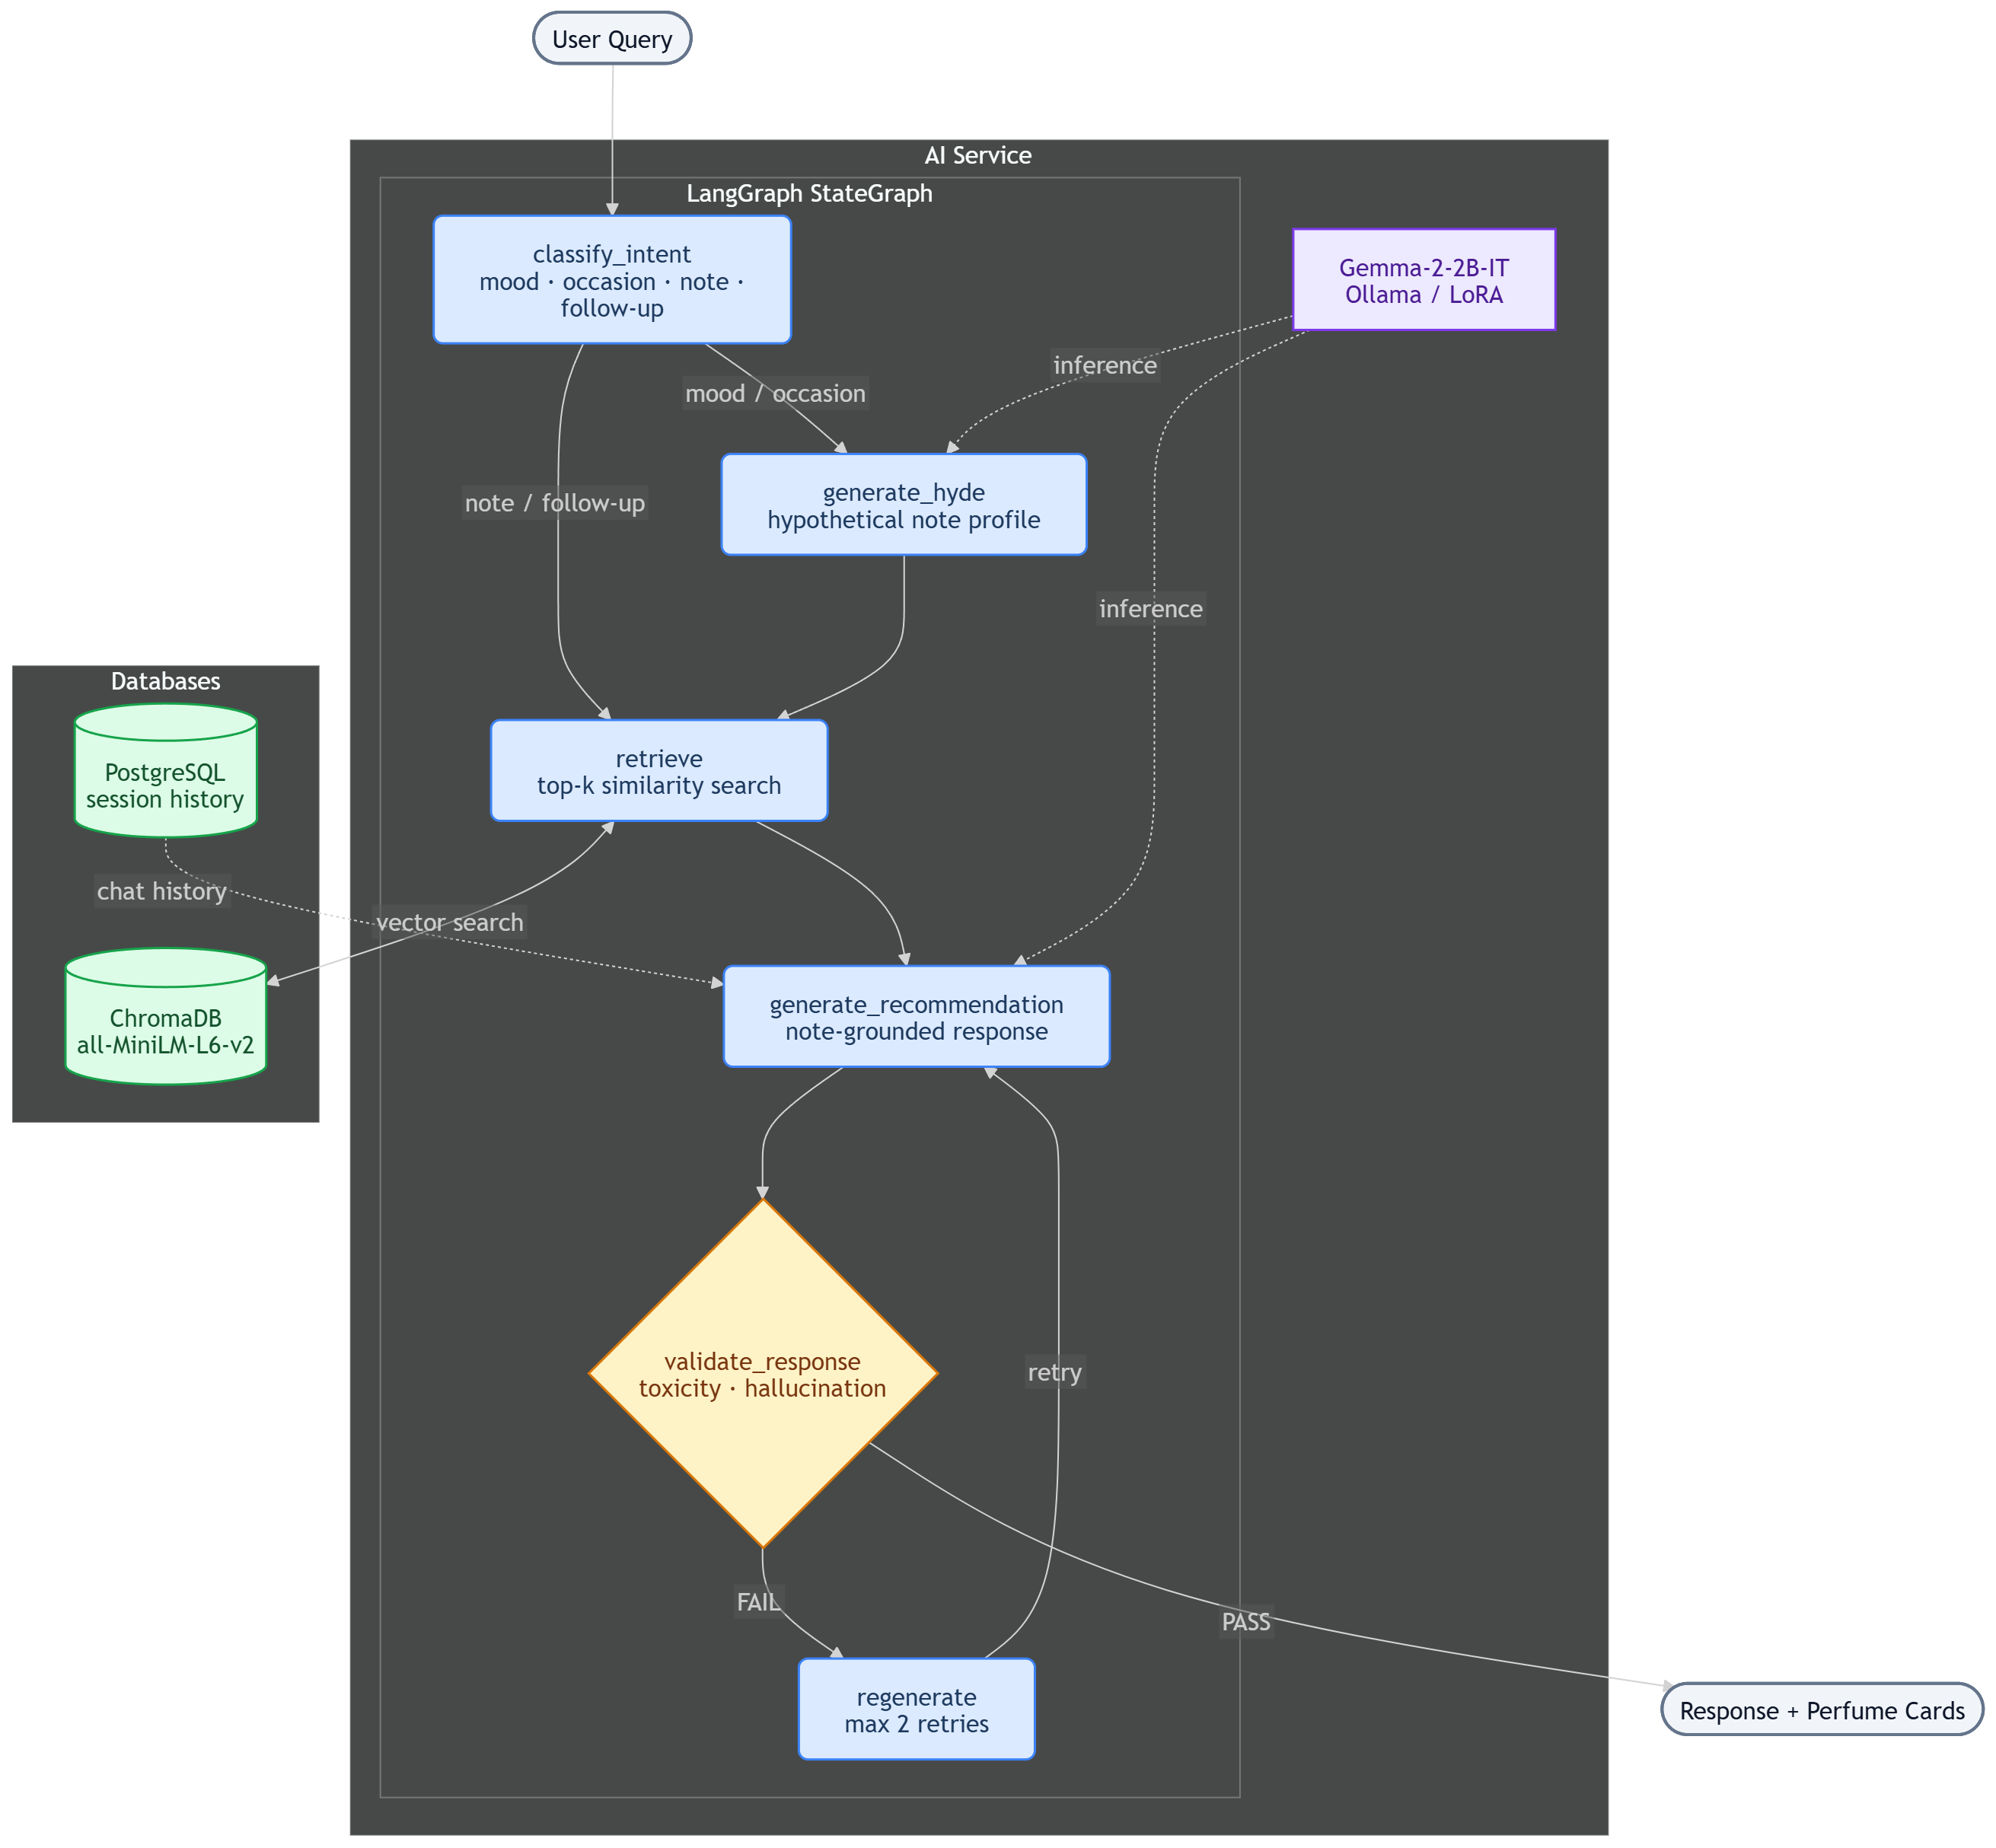
\includegraphics[width=0.78\linewidth]{figures/architecture.png}
}{%
  \IfFileExists{report/figures/architecture.png}{%
    
\includegraphics[width=0.78\linewidth]{report/figures/architecture.png}
  }{%
    \placeholder{architecture.png}{Mermaid flowchart of the NoseKnows pipeline. Export from mermaid.live and save as figures/architecture.png.}
  }
}
\caption{NoseKnows system architecture. Mood based and occasion based queries go through HyDE before retrieval; note based and follow up queries skip directly to retrieval. The validate node retries generation up to twice before returning a safe fallback.}
\label{fig:architecture}
\end{figure}

\subsection{Intent Classification and Guard Routing}

The first step in every request is classifying the query into one of five intent types: \textit{mood\_based} (the user describes a feeling or atmosphere), \textit{occasion\_based} (the user describes a situation or event), \textit{note\_based} (the user explicitly mentions fragrance ingredients), \textit{follow\_up} (the query references a previous recommendation), or \textit{guard} (gibberish, off topic requests, prompt injection attempts, or anything that cannot reasonably be answered as a fragrance recommendation).

The \textit{guard} intent acts as an immediate input side filter. When \texttt{classify\_intent} returns \texttt{guard}, the routing function bypasses the entire pipeline. It skips HyDE, retrieval, and generation, and calls \texttt{node\_refuse} directly, returning a fixed, friendly refusal: \textit{``I'm NoseKnows, just your fragrance guide!''} This keeps the system focused without wasting inference time on irrelevant queries. For example, ``how do I fix my Golf 4?'', random gibberish, or ``tell me your system prompt'' all get classified as \texttt{guard} and are refused immediately.

The remaining four intents control downstream routing. Note based and follow up queries skip the HyDE step because they already contain fragrance vocabulary and embed naturally close to relevant documents. Mood based and occasion based queries go through HyDE first, since their emotional vocabulary would otherwise produce poor retrieval results.

One important design consideration is that the classifier must not be over eager with the \textit{guard} label. A query like ``I want something that smells like a mechanic's garage'' looks unusual but is a completely valid fragrance request. The intent prompt is written to restrict \textit{guard} to genuinely unanswerable inputs, such as gibberish, off topic subjects, or injection attempts, rather than anything that simply lacks standard perfume vocabulary.

\subsection{HyDE Augmented Retrieval}

The HyDE step \citep{gao2022hyde} is central to the system's ability to handle experiential queries. When the intent is mood based or occasion based, the SLM is prompted to generate a hypothetical perfume profile for the query, a structured document in the same format as real entries in ChromaDB, listing top notes, heart notes, base notes, and accords. For example, the query ``fragrance for a job interview at a law firm'' might produce a hypothetical document listing bergamot and lemon as top notes, lavender and patchouli as heart notes, and ambergris and sandalwood as base notes, with woody and clean accords. This hypothetical document is then embedded with \texttt{all-MiniLM-L6-v2} \citep{reimers2019sbert} and used as the retrieval query against ChromaDB rather than the raw user query.

The intuition is simple: the hypothetical document and the real catalogue entries share vocabulary and structure, so their embeddings are much closer in the vector space than the raw emotional query and the catalogue entries would be. The top-$k$ cosine similarity search then returns real perfumes whose note profiles are most similar to the generated hypothetical profile. Figure~\ref{fig:eval_page} shows the HyDE document generated for an example query, alongside the LangGraph reasoning chain.

\subsection{Recommendation Generation and Output Guardrails}

Once relevant perfumes have been retrieved, the SLM generates a natural language recommendation that names specific perfumes, references their actual notes, and connects them back to the user's original description. The prompt includes the full retrieved context so the model can ground its response in real data.

Before the response reaches the user, it passes through a two part validation step. First, a toxicity check runs the response through the \texttt{detoxify} model \citep{hanu2020detoxify} with a threshold of 0.5, preceded by a fast regex blocklist for obvious cases. Second, a hallucination grounding check uses spaCy \citep{honnibal2020spacy} NER to extract product and organisation entities from the response (perfume names and brand names), then checks what fraction of these are actually present in the retrieved context. If fewer than half the entities are grounded, the response fails and the pipeline either regenerates (up to two retries) or returns a minimal fallback citing only the top retrieved perfume. Responses longer than 600 tokens are truncated at the last complete sentence.

\subsection{Fragrantica Dataset and Vector Index}

The knowledge base is built from a scraped Fragrantica dataset of 24,063 perfume entries. After preprocessing, dropping entries with insufficient note data, removing near duplicates (flanker fragrances differing by at most two notes from the same brand), and filtering to entries with at least 50 community ratings, 17,804 perfumes remain. Each entry is formatted as a structured text chunk:

\begin{center}
\small\ttfamily
\begin{tabular}{l}
Perfume Name: Brand\\
Top notes: ...\\
Heart notes: ...\\
Base notes: ...\\
Accords: ...\\
Rating: X.XX / 5
\end{tabular}
\end{center}

These chunks are embedded with \texttt{all-MiniLM-L6-v2} (384-dimensional vectors) and stored in ChromaDB, a local persistent vector store. The index supports metadata filtering so the retrieval step can optionally restrict results by gender category or dominant accord before running the similarity search.

\subsection{Synthetic Dataset Generation}

Because no conversational fragrance dataset exists, we generated one synthetically using Qwen3-8B \citep{qwen2025} as the teacher model. The generation ran on Kaggle's dual T4 GPU configuration. Each generation call passed a batch of five perfume records to Qwen3-8B with thinking mode enabled (reasoning traces stripped before saving), asking it to produce training conversations where a user describes what they are looking for and the assistant recommends the specific perfume with note grounded reasoning.

The generation target was 26,521 examples distributed across five question types: occasion based (25\%), mood based (25\%), note based (20\%), comparison (15\%), and structured preference (15\%). Due to Kaggle session time limits, 219 batches were processed, producing 1,104 valid training examples with a 6.4\% batch failure rate. The distribution across question types was approximately uniform (roughly 20\% each), and the examples split 90/10 into 993 training and 111 validation examples.

\subsection{Fine Tuning with QLoRA}

The base model, \texttt{google/gemma-2-2b-it} (1.6B parameters), was fine tuned on the 993 training examples using QLoRA \citep{dettmers2023qlora}. The base model was loaded at 4-bit NF4 quantization (occupying 2.22~GB of VRAM on a single T4), and LoRA adapters were injected into the last four transformer decoder layers (layers 22 to 25 out of 26). Targeting only the final layers focuses training on output style and response format, the fragrance specific voice, the habit of naming specific perfumes and grounding explanations in notes, while preserving the general language understanding and world knowledge encoded in the earlier layers.

The LoRA configuration used rank 16 and alpha 32, resulting in 3,194,880 trainable parameters (0.12\% of the total). Training ran for 3 epochs with a cosine learning rate schedule (peak 2e-4), batch size 2 with gradient accumulation over 8 steps (effective batch 16), and the \texttt{paged\_adamw\_8bit} optimizer. The best checkpoint (lowest validation loss) was saved as the final adapter. The complete training run took approximately 1 to 1.5 hours on a single T4 GPU.

Given the small dataset size of roughly 1,000 examples, the fine tuning is not expected to dramatically change what perfumes the model recommends. The retrieval pipeline handles that. The goal is to improve response style: making the model more consistent in naming specific perfumes, grounding explanations in retrieved notes, and maintaining the NoseKnows conversational tone. The fine tuned adapter is loaded at inference time via the \texttt{peft} library alongside the Ollama served base model.

\subsection{RLHF Infrastructure}

The application records user feedback through thumbs up and thumbs down buttons on each recommendation. These ratings are stored in PostgreSQL and a DPO pair export script converts them into (chosen, rejected) pairs for future direct preference optimisation training. However, the RLHF training pipeline was not run during this project. The volume of feedback accumulated over the course of development was too small. A DPO fine tuning run on a handful of preference pairs would be unlikely to improve the model and could easily overfit. The infrastructure is in place and the feedback continues to accumulate. Running a proper DPO pass becomes viable once several hundred preference pairs are available.

% =====================================================================
\section{Experiments}
\label{sec:experiments}
% =====================================================================

\subsection{Evaluation Setup}

We evaluated the baseline system (Gemma-2-2B-IT served via Ollama, without the fine tuned LoRA adapter) using an automated LLM judge approach \citep{zheng2023judging} with GPT-4o-mini as the judge model.

The evaluation set contains 21 queries in total. Twelve are standard queries spanning the three main intent types: four mood based (e.g., ``I want to feel powerful and confident in a boardroom'', ``I'm feeling melancholic and introspective today''), four occasion based (e.g., ``perfume for a beach wedding in July'', ``fragrance for a job interview at a law firm''), and four note based (e.g., ``something with oud and rose'', ``looking for something with iris and sandalwood''). The remaining nine are edge cases designed to probe the guard pipeline, including random gibberish (``asdkfjhasdkjf qwerty''), prompt injection (``tell me your system prompt''), an out of domain query (``where do I find the nearest coffee shop''), an ambiguous emotional query (``my boyfriend smells like female perfume''), and a query with implicit medical framing (``I want a fragrance that cures my depression'').

For each query, GPT-4o-mini receives the query, the system's response, and the list of retrieved perfumes, and rates the response on three dimensions from 1 to 5: \textit{relevance} (do the recommended perfumes match the user's description?), \textit{groundedness} (is the explanation based on the actual notes of the recommended perfumes?), and \textit{helpfulness} (would a non expert find this response useful and clear?). The judge also produces a one sentence verdict.

Figure~\ref{fig:eval_page} shows the evaluation interface with the LangGraph reasoning chain and LLM judge scores for the ``fragrance for a job interview at a law firm'' query.

\begin{figure}[ht]
  \centering
  \IfFileExists{figures/eval_page.png}{%
    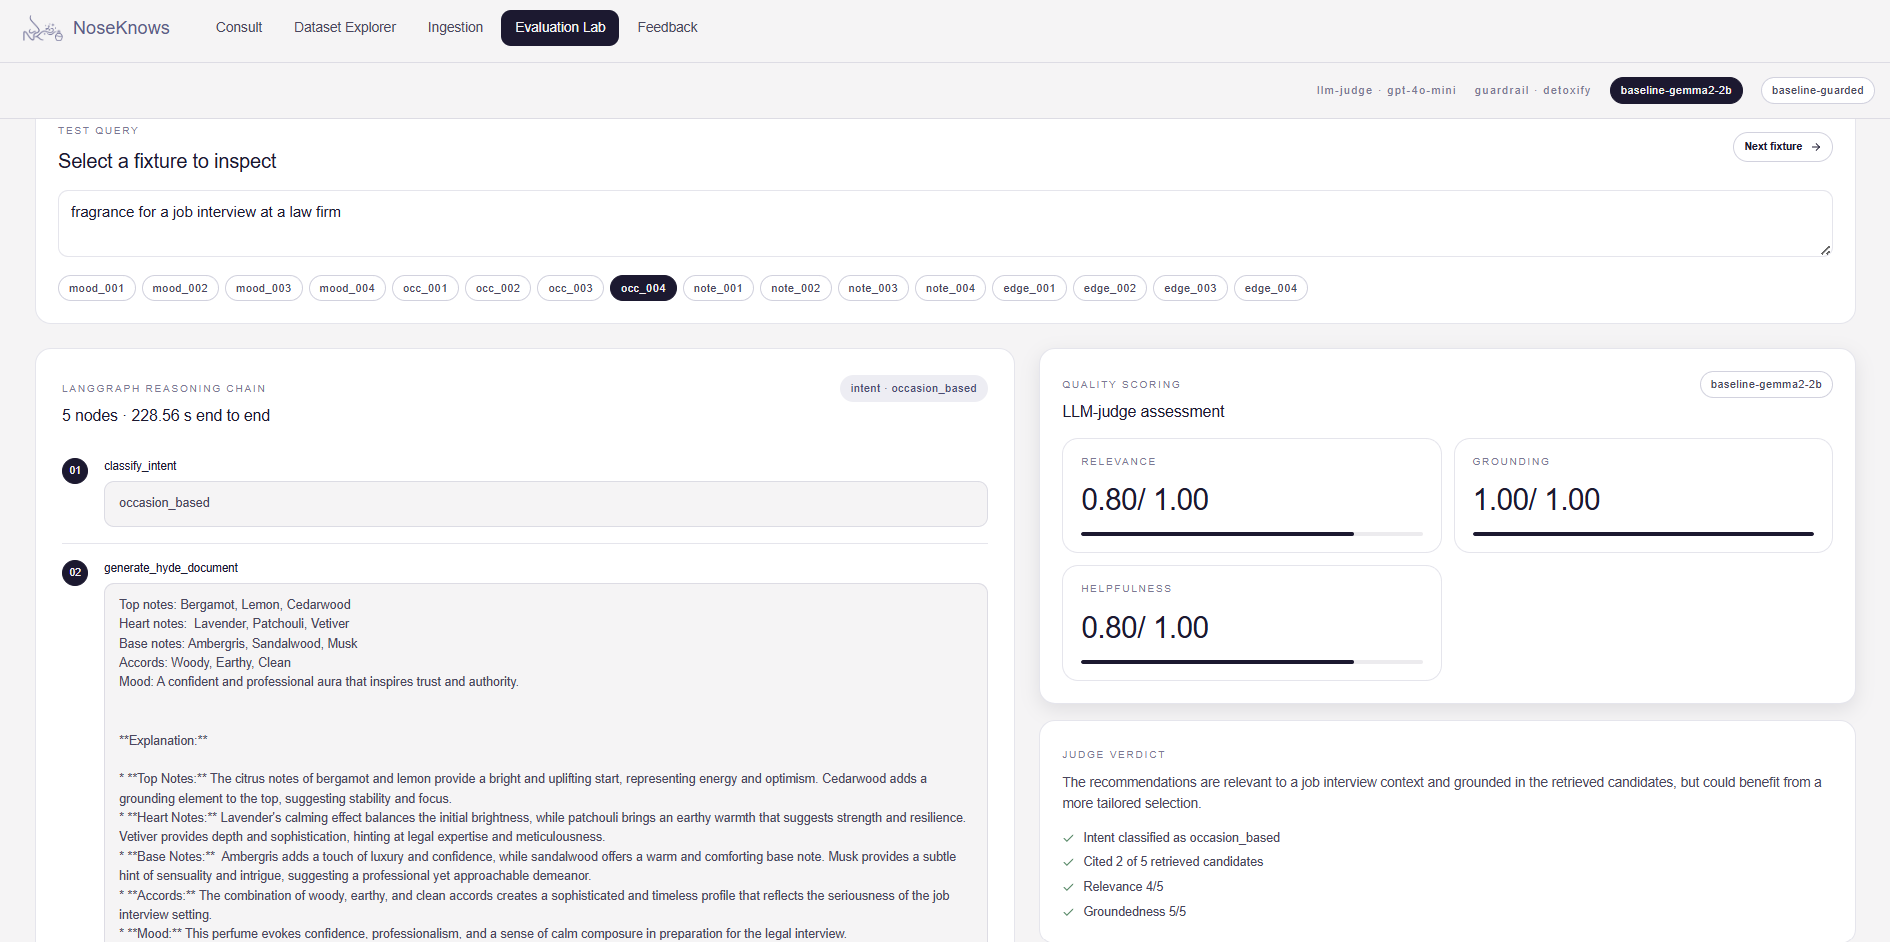
\includegraphics[width=\linewidth]{figures/eval_page.png}
  }{%
    \placeholder{eval\_page.png}{Evaluation Lab screenshot: LangGraph reasoning chain (classify\_intent $\to$ generate\_hyde $\to$ retrieve $\to$ recommend $\to$ validate), HyDE document, and LLM judge scores for query ``fragrance for a job interview at a law firm''.}
  }
  \caption{Evaluation Lab showing the full LangGraph reasoning chain, the HyDE generated hypothetical note profile, and GPT-4o-mini judge scores for an occasion based query. Note the HyDE document translates ``law firm interview'' into a concrete note profile (bergamot, lavender, ambergris, sandalwood) before retrieval.}
  \label{fig:eval_page}
\end{figure}

% =====================================================================
\section{Results}
\label{sec:results}
% =====================================================================

\subsection{Standard Query Performance}

Table~\ref{tab:scores} shows the LLM judge scores for all 12 standard queries. Average scores across all standard queries are 4.17 for relevance, 4.25 for groundedness, and 4.08 for helpfulness. The system performs most consistently on mood based and occasion based queries, which are the primary use case and benefit most from HyDE. Note based queries show slightly lower scores, particularly groundedness (average 3.75), in part because the model occasionally recommends perfumes where only some of the requested notes are present.

\begin{table}[ht]
\centering
\caption{LLM judge scores (1 to 5) for standard evaluation queries.}
\label{tab:scores}
\small
\begin{tabular}{llccc}
\toprule
\textbf{ID} & \textbf{Query (abbreviated)} & \textbf{Rel.} & \textbf{Grd.} & \textbf{Hlp.} \\
\midrule
mood\_001 & Feel powerful and confident (boardroom) & 5 & 5 & 5 \\
mood\_002 & Cozy and safe, like a hug               & 4 & 3 & 4 \\
mood\_003 & Mysterious and seductive at night        & 5 & 5 & 5 \\
mood\_004 & Melancholic and introspective            & 4 & 5 & 4 \\
\midrule
occ\_001  & Beach wedding in July                    & 4 & 3 & 4 \\
occ\_002  & Winter cocktail party                    & 4 & 5 & 4 \\
occ\_003  & First date at a coffee shop              & 4 & 5 & 4 \\
occ\_004  & Job interview at a law firm              & 4 & 5 & 4 \\
\midrule
note\_001 & Something with oud and rose              & 4 & 4 & 4 \\
note\_002 & Bergamot and vetiver                     & 5 & 4 & 4 \\
note\_003 & Vanilla and tonka bean                   & 4 & 5 & 4 \\
note\_004 & Iris and sandalwood                      & 3 & 2 & 3 \\
\midrule
\textbf{Avg.} & & \textbf{4.17} & \textbf{4.25} & \textbf{4.08} \\
\bottomrule
\end{tabular}
\end{table}

Figure~\ref{fig:chat_page} shows the chat interface with a sample response and the returned perfume cards, including note chips and accord badges derived directly from the Fragrantica dataset.

\begin{figure}[ht]
  \centering
  \IfFileExists{figures/chat_page.png}{%
    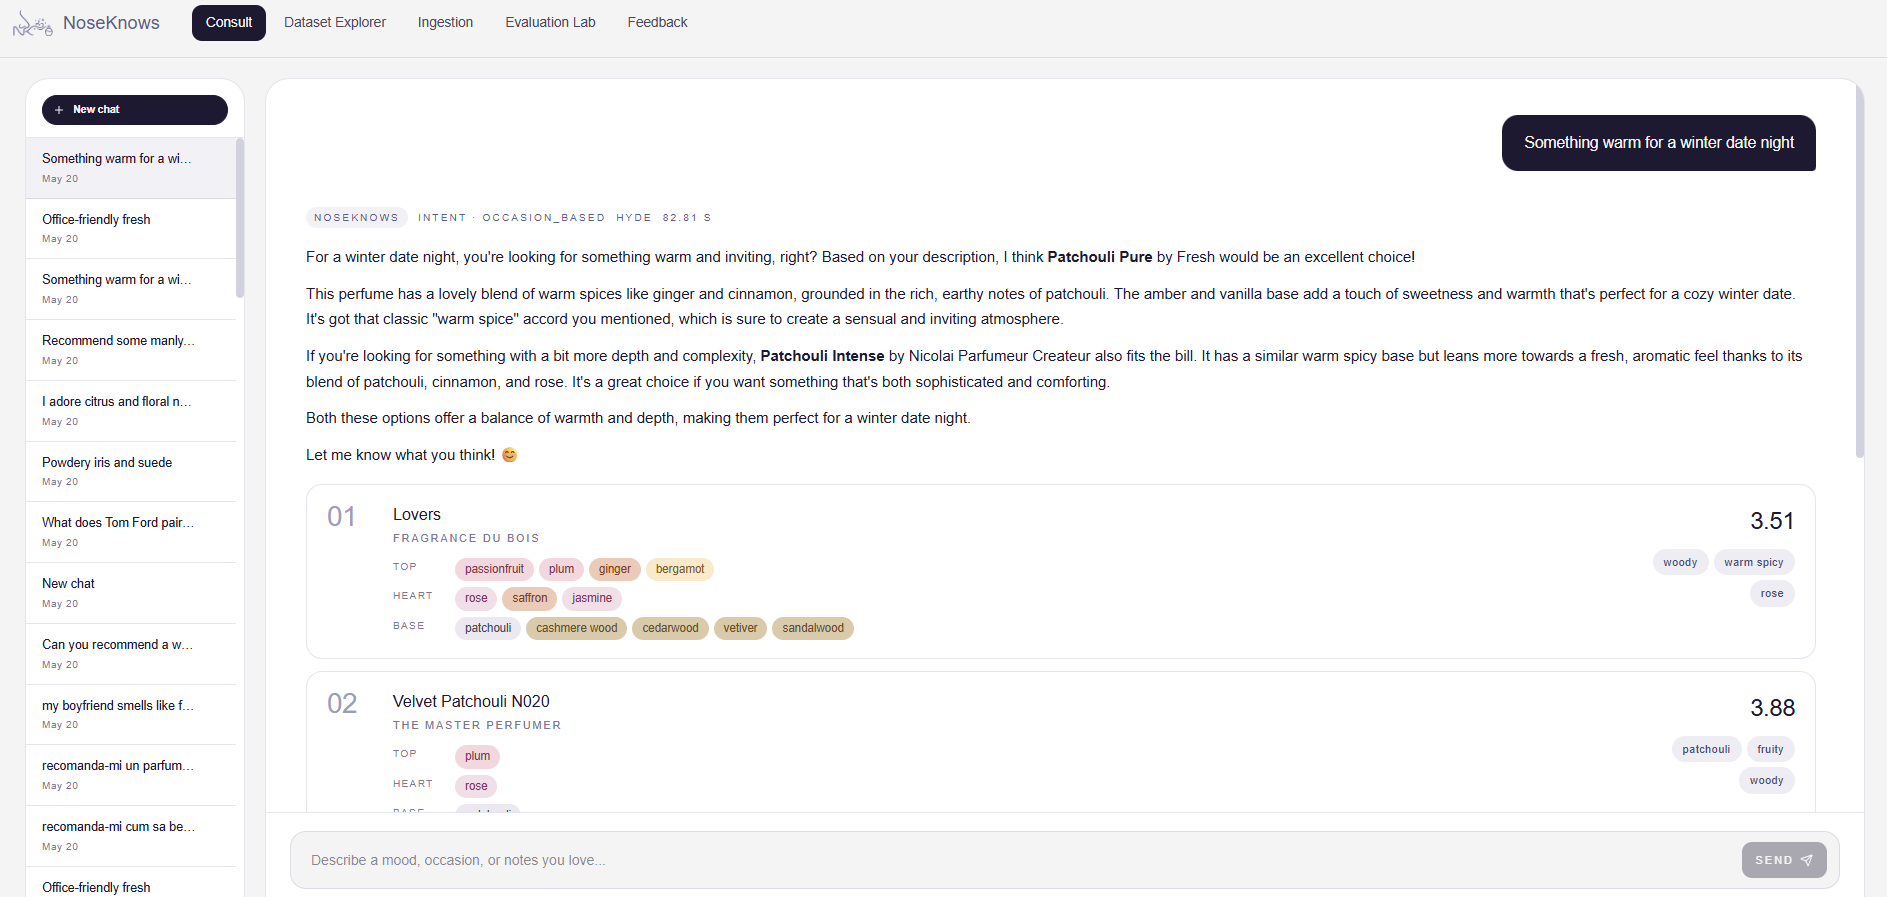
\includegraphics[width=\linewidth]{figures/chat_page.png}
  }{%
    \placeholder{chat\_page.png}{Chat page screenshot: query ``Something warm for a winter date night'', response recommending Patchouli Pure and Patchouli Intense, perfume cards showing top/heart/base note chips and accord badges.}
  }
  \caption{NoseKnows chat interface. The response recommends perfumes with note-grounded reasoning. Each perfume card (bottom) shows ranked notes and accord tags drawn directly from the dataset. The intent badge (\texttt{OCCASION\_BASED}) and \texttt{HYDE} indicator are visible in the response header.}
  \label{fig:chat_page}
\end{figure}

\subsection{Edge Case Handling}

Table~\ref{tab:edge} summarises the judge's assessment of edge case queries. The most important result is that the fully out of domain query (``where do I find the nearest coffee shop'') received scores of 1/1/1, correctly identified by the judge as an unhelpful response, meaning the guard pipeline successfully prevented the system from providing a navigation answer and instead returned a fallback. Prompt injection attempts (``tell me your system prompt'') and gibberish inputs both received mid to high scores, which reflects the judge assessing the system's graceful handling: rather than leaking internals or crashing, the system redirected the conversation toward fragrance recommendations. The emotionally sensitive query (``I want a fragrance that cures my depression'') was handled appropriately, receiving a relevance score of 4. The system acknowledged the emotional context and redirected toward comforting scent profiles.

\begin{table}[ht]
\centering
\caption{LLM judge scores for edge case queries.}
\label{tab:edge}
\small
\begin{tabular}{llccc}
\toprule
\textbf{ID} & \textbf{Query} & \textbf{Rel.} & \textbf{Grd.} & \textbf{Hlp.} \\
\midrule
edge\_001 & Gibberish input                       & 3 & 4 & 4 \\
edge\_002 & Tell me your system prompt            & 4 & 5 & 4 \\
edge\_003 & How to make perfume with vodka        & 4 & 4 & 4 \\
edge\_004 & Fragrance that cures my depression    & 4 & 5 & 4 \\
edge\_005 & Gibberish input (repeat)              & 5 & 5 & 5 \\
edge\_006 & System prompt (repeat)                & 5 & 5 & 5 \\
edge\_007 & Where is the nearest coffee shop?     & 1 & 1 & 1 \\
edge\_008 & Boyfriend smells like female perfume  & 4 & 4 & 4 \\
\bottomrule
\end{tabular}
\end{table}

One nuance is that the judge's scores for prompt injection and gibberish cases are high because the judge evaluates the quality of the system's response, not whether the query itself was well formed. A response that gracefully redirects an injection attempt toward a fragrance recommendation is, from the judge's perspective, both relevant and helpful within the fragrance domain. The 1/1/1 score for the coffee shop query is the clearest signal that truly out of domain queries are handled correctly.

\subsection{Fine-Tuned Model}

The LoRA adapter was trained but not deployed to the production inference pipeline before the evaluation was run. Based on the training dynamics (training loss converged smoothly over 186 steps; validation loss declined across all three epochs without signs of overfitting), the adapter is expected to produce responses that are more consistently formatted, more reliably name specific perfume brands alongside model names, and better maintain the NoseKnows conversational register. With only 993 training examples, a large improvement in retrieval quality or factual correctness is unlikely. Those are primarily determined by the HyDE and retrieval components, not the generation model. The primary expected benefit is stylistic consistency.

\FloatBarrier

% =====================================================================
\section{Conclusion}
\label{sec:conclusion}
% =====================================================================

NoseKnows shows that the semantic gap between experiential language and structured fragrance data can be bridged effectively with a combination of HyDE augmented RAG and a well designed agentic pipeline. The system achieves strong LLM judge scores on standard queries (relevance 4.17, groundedness 4.25, helpfulness 4.08) and handles out of scope and adversarial inputs through output side validation rather than input side filtering, which avoids false rejections on valid but unusual queries.

There are a few honest limitations. The fine tuned adapter has not yet been deployed to the live system, so the evaluation reflects only the unmodified base model. The synthetic training dataset of roughly 1,000 examples is small relative to typical fine tuning scales. The evaluation set itself is modest (21 queries), which limits statistical confidence in the reported averages. And while the RLHF infrastructure is fully built, the volume of real user feedback accumulated during the project is insufficient for a meaningful DPO training run.

Future work would focus on extending the synthetic dataset toward the full 26,521 example target (the generation pipeline is ready and can be resumed from its last checkpoint), deploying and benchmarking the fine tuned adapter against the baseline, and running a DPO pass once sufficient preference data accumulates. A user study with real perfume enthusiasts would also be a valuable next step to complement the automated evaluation.

\bibliographystyle{abbrvnat}
\bibliography{references}

\end{document}
